\documentclass[11pt,a4paper]{article}

\usepackage[utf8]{inputenc}
\usepackage{geometry}
\usepackage[colorlinks=true, linkcolor=blue, urlcolor=blue, citecolor=blue]{hyperref}
\usepackage{booktabs}
\usepackage{enumitem}
\usepackage{graphicx}
\usepackage{float}
\usepackage{xcolor}
\usepackage{tabularx}
\usepackage{array}
\usepackage{parskip}
\usepackage{titlesec}
\usepackage{fancyhdr}
\usepackage{setspace}
\usepackage{mdframed}
\usepackage{tcolorbox}

\geometry{top=1in, bottom=1in, left=1.2in, right=1.2in}
\setstretch{1.15}

% Header / footer
\pagestyle{fancy}
\fancyhf{}
\rhead{COM 763 Advanced Machine Learning}
\lhead{Portfolio Task 2 --- Model Card}
\cfoot{\thepage}
\renewcommand{\headrulewidth}{0.4pt}

% Section formatting
\titleformat{\section}{\large\bfseries}{\thesection.}{1em}{}[\titlerule]
\titleformat{\subsection}{\normalsize\bfseries}{\thesubsection}{1em}{}

% Coloured box for key info panels
\tcbuselibrary{skins,breakable}
\newtcolorbox{infobox}[2][]{
  colback=blue!5!white, colframe=blue!50!black,
  title=#2, fonttitle=\bfseries, #1
}

% ----------------------------------------------------------------
\title{%
  \vspace{-1cm}
  \textbf{COM 763 Advanced Machine Learning}\\[0.5em]
  \large Portfolio Task 2: Model Card\\[0.3em]
  \LARGE\bfseries Wine Quality Predictor
}
\author{Student ID: [Your ID] \\ Wrexham University}
\date{\today}
% ----------------------------------------------------------------

\begin{document}

\maketitle
\thispagestyle{empty}

\vspace{0.5em}
\begin{center}
\begin{tabular}{ll}
  \textbf{Model Version:}   & 1.0.0 \\
  \textbf{Model Type:}      & Random Forest Classifier \\
  \textbf{Task:}            & Binary Classification \\
  \textbf{Domain:}          & Food \& Beverage Quality Assurance \\
  \textbf{Deployment:}      & \url{https://proect-wine.streamlit.app} \\
  \textbf{Repository:}      & \url{https://github.com/[your-username]/Proect-Wine} \\
  \textbf{Last Updated:}    & August 2026 \\
\end{tabular}
\end{center}

\vspace{1em}
\hrule
\vspace{0.5em}

\tableofcontents
\newpage

% ================================================================
\section{Model Overview and Intended Use}
% ================================================================

\subsection{High-Level Description}

The \textbf{Wine Quality Predictor} is a machine learning classification model designed to automate a key step in wine production quality control. Given a set of eleven standard physicochemical measurements taken from a wine sample, the model predicts whether the wine will be perceived as \textbf{``Good Quality''} (corresponding to a sensory score of 6 or above on a 10-point scale) or \textbf{``Bad Quality''} (a score below 6).

The model addresses a real and costly challenge in the wine industry: the reliance on subjective, expensive, and slow human expert tasting to evaluate production batches. By leveraging chemical analysis data that is routinely collected during production, the system provides a rapid, consistent, and objective quality estimate that can complement human judgement.

The model was developed as part of an academic machine learning portfolio at Wrexham University (Module: COM 763, Advanced Machine Learning) and is deployed as an interactive web application on Streamlit Community Cloud.

\begin{infobox}{System at a Glance}
  \begin{tabular}{ll}
    \textbf{Input:}   & 11 continuous physicochemical measurements \\
    \textbf{Output:}  & Binary label (Good Quality / Bad Quality) \\
    \textbf{Algorithm:}  & Random Forest Classifier (100 trees) \\
    \textbf{Training Data:} & WineQT dataset (1,143 red wine samples) \\
    \textbf{Interface:}  & Streamlit web application with interactive sliders \\
  \end{tabular}
\end{infobox}

\subsection{Intended Users and Deployment Context}

This system is designed to be used by the following groups:

\begin{itemize}[leftmargin=*]
    \item \textbf{Wine Producers and Vineyard Managers:} As a rapid, preliminary screening tool during the fermentation and production process. A producer can enter the latest chemical assay results into the application and receive an immediate quality estimate, allowing them to identify problematic batches early and make corrective interventions (e.g., adjusting sulphate additions or controlling alcohol fermentation).

    \item \textbf{Quality Assurance Technicians:} As a secondary check to flag borderline samples that may warrant a closer examination by a human taster, helping to prioritise the workload of the tasting panel.

    \item \textbf{Academic and Research Contexts:} As a demonstration of a complete, end-to-end machine learning pipeline applied to the food science domain.
\end{itemize}

The system is designed to function as a \textbf{decision-support tool}, not as an autonomous decision-maker. All predictions should be reviewed by a qualified human before any significant production or commercial decision is made based on them.

\subsection{Intended Use Cases}

\begin{itemize}[leftmargin=*]
    \item Rapid preliminary quality screening of production batches during the winemaking process.
    \item Prioritising wine samples for full sensory tasting panels based on model confidence scores.
    \item Educating production staff on the chemical factors most strongly associated with perceived wine quality.
    \item Quality monitoring over time: tracking trends in predicted quality scores across production seasons.
\end{itemize}

\subsection{Non-Intended Uses}

The following uses are \textbf{explicitly out of scope} and are considered inappropriate applications of this model:

\begin{itemize}[leftmargin=*]
    \item \textbf{Final pricing or commercial grading decisions:} The model should not be used as the sole determinant for setting retail prices or assigning premium/standard labels to wine products.
    \item \textbf{Replacing expert tasters for premium wines:} For high-value, artisanal, or competition wines where subtle sensory nuances (aroma complexity, finish, mouthfeel) are paramount, human expert evaluation remains essential. These attributes are not captured by the model's input features.
    \item \textbf{White wine or sparkling wine assessment:} The model was trained exclusively on red wine data. Applying it to white wines or other wine styles is likely to produce unreliable results.
    \item \textbf{Regulatory compliance assessment:} This tool is not validated for use in any official food safety, labelling, or regulatory certification context.
    \item \textbf{Detecting specific wine faults or contaminants:} The model predicts an overall quality category and is not designed to identify specific defects such as cork taint, oxidation from specific sources, or bacterial contamination.
\end{itemize}

% ================================================================
\section{System and Data Summary}
% ================================================================

\subsection{Model Architecture}

The core model is a \textbf{Random Forest Classifier} from the Scikit-learn machine learning library (Python). A Random Forest is an \textit{ensemble} method that builds many individual decision trees during training and combines their predictions to produce a final output. This approach makes the model significantly more robust and accurate than any single decision tree.

The model was selected over a Logistic Regression baseline after a rigorous experimental comparison (detailed in Section~\ref{sec:evaluation}) demonstrated its superior performance on all key metrics.

\begin{table}[H]
    \centering
    \caption{Key System Parameters}
    \label{tab:params}
    \begin{tabular}{ll}
        \toprule
        \textbf{Parameter} & \textbf{Value} \\
        \midrule
        Algorithm & Random Forest Classifier \\
        Number of Trees (\texttt{n\_estimators}) & 100 \\
        Maximum Tree Depth (\texttt{max\_depth}) & Unconstrained \\
        Minimum Samples to Split (\texttt{min\_samples\_split}) & 2 \\
        Tuning Method & 5-fold Cross-Validation GridSearchCV \\
        Feature Preprocessing & StandardScaler (z-score normalisation) \\
        Serialisation Format & joblib \\
        Deployment Framework & Streamlit \\
        \bottomrule
    \end{tabular}
\end{table}

\subsection{Input and Output Description}

\textbf{Inputs:} The model accepts eleven continuous numerical features, all of which are standard measurements in physicochemical wine analysis:

\begin{table}[H]
    \centering
    \caption{Model Input Features}
    \label{tab:inputs}
    \begin{tabularx}{\textwidth}{lX}
        \toprule
        \textbf{Feature} & \textbf{Typical Range / Units} \\
        \midrule
        Fixed Acidity & 4.0 -- 16.0 g/dm\textsuperscript{3} \\
        Volatile Acidity & 0.1 -- 1.6 g/dm\textsuperscript{3} \\
        Citric Acid & 0.0 -- 1.0 g/dm\textsuperscript{3} \\
        Residual Sugar & 0.5 -- 16.0 g/dm\textsuperscript{3} \\
        Chlorides & 0.01 -- 0.60 g/dm\textsuperscript{3} \\
        Free Sulfur Dioxide & 1 -- 72 mg/dm\textsuperscript{3} \\
        Total Sulfur Dioxide & 6 -- 290 mg/dm\textsuperscript{3} \\
        Density & 0.990 -- 1.005 g/cm\textsuperscript{3} \\
        pH & 2.5 -- 4.1 \\
        Sulphates & 0.3 -- 2.0 g/dm\textsuperscript{3} \\
        Alcohol & 8.0 -- 15.0 volume \\
        \bottomrule
    \end{tabularx}
\end{table}

\textbf{Outputs:} The model produces two outputs:
\begin{itemize}[leftmargin=*]
    \item A \textbf{binary class label}: \texttt{1} (Good Quality) or \texttt{0} (Bad Quality).
    \item A \textbf{probability score} (0.0 -- 1.0) representing the model's confidence that the wine falls into the ``Good Quality'' category. A score of 0.85, for example, indicates high confidence the wine is good quality.
\end{itemize}

\subsection{Training Data Summary}

The model was trained on the \textbf{WineQT dataset}, which contains 1,143 records of physicochemical analyses of red (Vinho Verde) wines from Portugal, paired with quality scores from expert sensory evaluations. The dataset is openly available and is a standard benchmark in the machine learning literature.

\textbf{Key assumptions about the data:}
\begin{itemize}[leftmargin=*]
    \item The chemical measurements are assumed to have been collected using standardised, calibrated laboratory instruments, ensuring measurement consistency.
    \item The quality scores in the training data represent an average or consensus view from multiple human tasters, not a single individual's judgement.
    \item All samples in the dataset are red wines from a specific Portuguese wine-producing region (Vinho Verde), which defines the distributional scope of the model.
\end{itemize}

% ================================================================
\section{Evaluation and Performance Summary}
\label{sec:evaluation}
% ================================================================

\subsection{Evaluation Approach}

The model was evaluated using a \textbf{held-out test set} comprising 229 wine samples (approximately 20\% of the full dataset) that were set aside before any model training began. This ensures that the reported performance reflects the model's ability to generalise to genuinely unseen data, rather than simply its ability to memorise training examples.

To select the best model configuration, \textbf{5-fold cross-validation} was applied during the hyperparameter tuning phase. In 5-fold cross-validation, the training data is split into five equal parts; the model is trained on four parts and evaluated on the fifth, and this process is repeated five times. This provides a more robust estimate of model performance than a single train-validate split.

\subsection{Performance Results}

\begin{table}[H]
    \centering
    \caption{Model Performance on Hold-out Test Set}
    \label{tab:perf}
    \begin{tabular}{lcccc}
        \toprule
        \textbf{Model} & \textbf{Accuracy} & \textbf{Precision} & \textbf{Recall} & \textbf{F1-Score} \\
        \midrule
        Logistic Regression (Baseline) & 0.773 & 0.802 & 0.782 & 0.792 \\
        \textbf{Random Forest (Final)} & \textbf{0.808} & \textbf{0.809} & \textbf{0.855} & \textbf{0.831} \\
        \bottomrule
    \end{tabular}
\end{table}

In plain terms, the final Random Forest model correctly classifies approximately \textbf{8 out of 10 wine samples} in the test set. More importantly, when a wine is truly of good quality, the model correctly identifies it as such roughly \textbf{85 out of every 100 times} (Recall = 0.855), meaning very few good wines are incorrectly rejected.

The model's ROC-AUC score of \textbf{0.87} (compared to 0.82 for the baseline) indicates strong discriminative ability. This means the model can reliably rank wine samples such that truly good wines receive higher predicted probability scores than truly bad wines.

\begin{figure}[H]
    \centering
    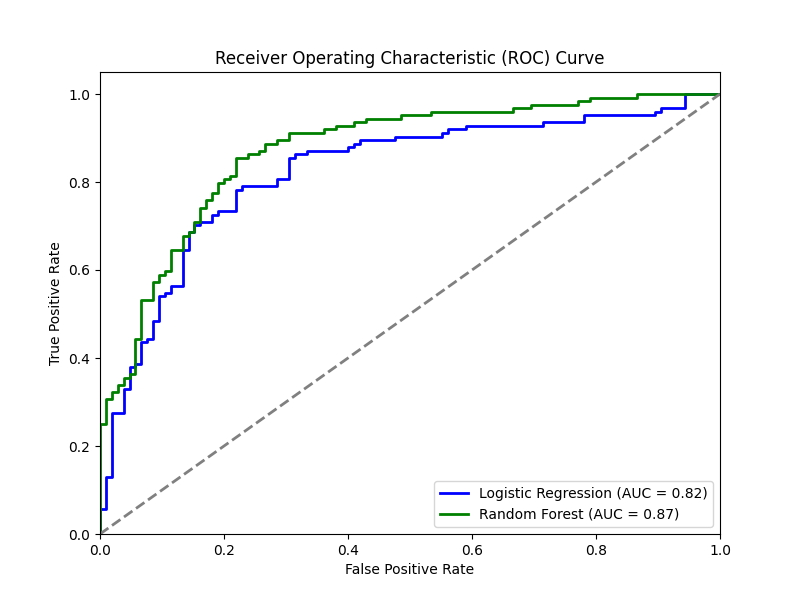
\includegraphics[width=0.8\textwidth]{figures/roc_curves.png}
    \caption{ROC curves comparing the Logistic Regression baseline and the final Random Forest model. A higher curve (closer to the top-left corner) indicates better discriminative performance. The Random Forest (green, AUC = 0.87) clearly outperforms the baseline (blue, AUC = 0.82).}
    \label{fig:roc2}
\end{figure}

\begin{figure}[H]
    \centering
    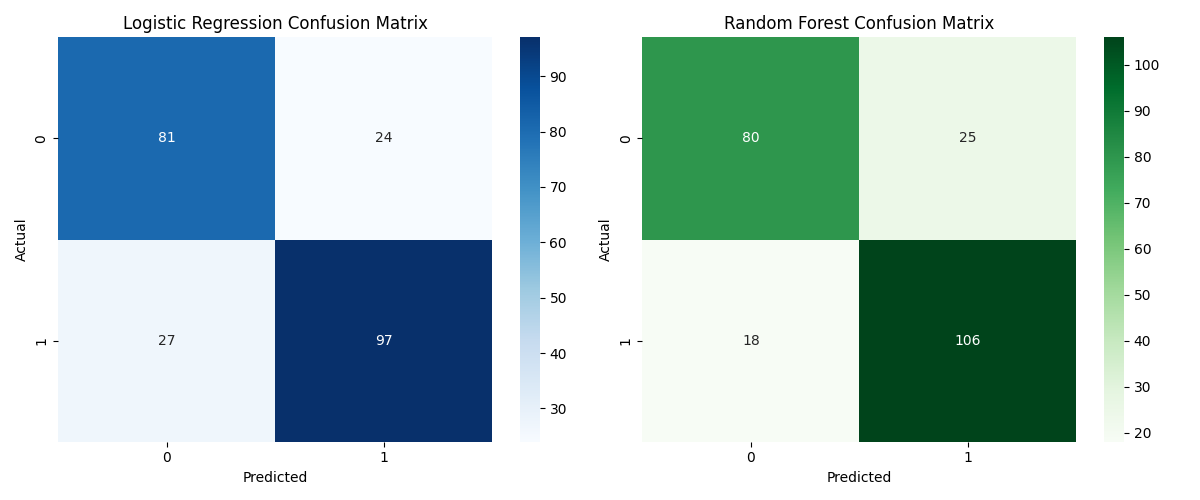
\includegraphics[width=\textwidth]{figures/confusion_matrices.png}
    \caption{Confusion matrices showing the breakdown of correct and incorrect predictions for both models on the test set. The Random Forest (right) produces notably fewer false negatives (18 vs.\ 27), meaning it misses fewer genuinely good wines.}
    \label{fig:cm2}
\end{figure}

\subsection{Key Predictive Factors}

Analysis of the model reveals the chemical properties most strongly associated with wine quality:

\begin{enumerate}[leftmargin=*]
    \item \textbf{Alcohol content} is the single most important predictor, followed by \textbf{sulphates} and \textbf{volatile acidity}. These findings are consistent with established oenological knowledge.
    \item Wines with \textbf{higher alcohol} and \textbf{appropriate sulphate levels}, combined with \textbf{low volatile acidity}, are most likely to be rated as ``Good Quality.''
\end{enumerate}

\subsection{Limitations of the Evaluation}

\begin{itemize}[leftmargin=*]
    \item \textbf{Dataset size:} The test set comprises only 229 samples. While this is standard for this dataset, a larger evaluation set would produce more statistically robust performance estimates.
    \item \textbf{Distribution shift:} The evaluation reflects performance on wines from the same distribution as the training data (Portuguese Vinho Verde red wine). Performance on wines from other regions, grape varieties, or production methods is unknown.
    \item \textbf{Temporal validity:} The dataset does not include timestamps for the wine samples. If production methods or taster preferences have changed over time, the model's real-world performance could degrade without retraining.
    \item \textbf{Threshold sensitivity:} The binary classification threshold (0.5 probability) was used for reporting the metrics in Table~\ref{tab:perf}. Adjusting this threshold could improve Precision at the expense of Recall, or vice versa, depending on the specific business requirement.
\end{itemize}

% ================================================================
\section{Limitations, Risks, and Responsible Use}
% ================================================================

\subsection{Known Technical Limitations}

\begin{itemize}[leftmargin=*]
    \item \textbf{Subjectivity of the Target Variable:} The model was trained to predict the \textit{average human quality score}, which is itself a subjective and imperfect measure. The model does not have access to the individual taster scores or the level of agreement between tasters. Wines that divide opinion among experts are likely to be the most challenging for the model to classify correctly.

    \item \textbf{Limited Feature Set:} The eleven chemical features available do not capture all factors that influence perceived wine quality. Factors such as the wine's vintage year, the grape variety, the specific terroir (soil composition, microclimate), the winemaking process (oak ageing, yeast strain), and the condition of the bottle at tasting are all absent from the model's input.

    \item \textbf{Boundary Uncertainty:} Wines with quality scores of exactly 5 or 6 are the most ambiguous cases, as they fall near the ``Good''/``Bad'' boundary. The model will have the most uncertainty and the highest error rate for samples in this borderline zone, which constitutes a substantial proportion of the dataset.

    \item \textbf{Scope Limited to Red Wine:} All training data comes from red wine samples. The model should not be used for white wines, ros\'{e} wines, or fortified wines, as their chemical profiles and the relationship between chemistry and quality may differ substantially.
\end{itemize}

\subsection{Risks and Potential Misuse}

\begin{itemize}[leftmargin=*]
    \item \textbf{Risk: Over-reliance and automation bias.} There is a risk that users, particularly those under time pressure, might accept the model's predictions uncritically, especially when the model has high stated confidence. This is known as \textit{automation bias}. For example, a batch of wine with subtle microbial contamination not detectable through standard chemical testing might be incorrectly labelled as ``Good Quality.''

    \textit{Mitigation:} The application clearly states the model's limitations and frames its output as a \textit{support tool}. Users should be trained to understand that high model confidence does not guarantee quality.

    \item \textbf{Risk: Geographical and dataset bias.} The model was trained exclusively on data from the Vinho Verde region of Portugal. Wines from other geographical regions --- even of identical chemical composition --- may carry different quality associations due to regional taster preferences, different grape varieties, or different production traditions. Applying the model to non-Portuguese wines without retraining could produce systematically biased results.

    \textit{Mitigation:} Documentation clearly states the geographical scope of the model. Users producing wines from other regions should retrain or fine-tune the model on locally-relevant data.

    \item \textbf{Risk: Economic harm from false predictions.} A False Positive prediction (labelling a bad wine as good) could result in substandard wine being released to market, damaging a producer's reputation. A False Negative prediction (labelling a good wine as bad) could result in unnecessary waste of a profitable product.

    \textit{Mitigation:} Any batch flagged as ``Bad'' by the model should be subject to a mandatory human tasting review before being discarded. The model should not be the sole reason for discarding wine.

    \item \textbf{Risk: Amplification of historical biases.} If the human tasters who assigned quality scores in the training data held implicit biases (e.g., preferences for a particular style of wine), the model will learn and perpetuate those biases in its predictions.

    \textit{Mitigation:} Periodic auditing of the model's predictions against diverse panels of expert tasters is recommended to identify and correct for any systematic bias.
\end{itemize}

\subsection{Ethical and Societal Considerations}

This model operates in the food and beverage sector, where its primary stakeholders are producers, quality assurance professionals, and ultimately consumers. The following ethical considerations are relevant:

\begin{itemize}[leftmargin=*]
    \item \textbf{Consumer Trust:} Wines marketed as ``premium quality'' based on a model prediction, without adequate human verification, could mislead consumers if the model is incorrect. Producers have an ethical obligation to ensure that quality claims are substantiated.

    \item \textbf{Impact on skilled workers:} The automation of quality assessment tasks, if adopted at scale, could reduce the demand for human tasting expertise. This has implications for wine professionals and the broader craft traditions of the industry. The model is designed as a supplement, not a replacement, for human skill.

    \item \textbf{Environmental footprint:} From a sustainability perspective, reducing wine waste by more accurately identifying quality issues early in production is a positive societal outcome, reducing resource consumption associated with producing, bottling, and discarding below-standard wine.

    \item \textbf{Small producer accessibility:} A freely accessible web application democratises access to data-driven quality insights, which could particularly benefit small producers who cannot afford large tasting panels.
\end{itemize}

\subsection{Responsible Deployment Guidelines}

To use this model responsibly, the following practices are strongly recommended:

\begin{enumerate}[leftmargin=*]
    \item Always treat model predictions as one data point among several, not as a definitive verdict.
    \item Maintain a mandatory human review step for all commercially significant decisions.
    \item Continuously monitor the model's predictions against actual quality outcomes in production to detect performance drift.
    \item Retrain the model periodically as new, locally-relevant data becomes available.
    \item Clearly communicate the model's geographical and dataset limitations to all end-users.
    \item Never use the model for regulatory, legal, or certification purposes.
\end{enumerate}

% ================================================================
\section{Presentation and Communication Quality}
% ================================================================

\subsection{Summary of Key Findings}

This Model Card provides a transparent, structured, and honest disclosure of the Wine Quality Predictor's capabilities and limitations. The most important points for a prospective user to understand are:

\begin{itemize}[leftmargin=*]
    \item The model performs well on wines chemically similar to those in the Vinho Verde (Portugal) red wine training dataset, correctly classifying approximately 8 in 10 samples.
    \item The model's predictive power is driven primarily by alcohol content, sulphates, and volatile acidity --- a finding that aligns with established oenological principles.
    \item The model is a \textbf{decision-support tool} and must not be used as the sole basis for commercial or regulatory decisions.
    \item Users outside the model's training distribution (different regions, wine types) should exercise significant caution and should consider retraining the model on representative local data.
\end{itemize}

\subsection{Further Information}

\begin{itemize}[leftmargin=*]
    \item For the full technical development narrative, including implementation details, debugging logs, and step-by-step evaluation, please refer to the accompanying Portfolio Task 1 Technical Report.
    \item The complete source code, Jupyter notebook (\texttt{.ipynb}), and all trained model artefacts are available in the project's GitHub repository: \url{https://github.com/[your-username]/Proect-Wine}.
    \item The live interactive application can be accessed at: \url{https://proect-wine.streamlit.app}.
\end{itemize}

\end{document}
